\subsection{The Business Model}

There are primarily two ways of monetizing a product such as ours: Selling the
product to our end users, or selling our end users to other companies. The
former would typically involve a subscription fee, which would require users
to authenticate themselves prior to using the service, and/or charging a
one-time fee for our mobile apps. Selling our end users might mean showing
advertisements in our trip planner, or taking a commission on the sale of
tickets.

Each of these models have their pros and cons. Charging customers to use our
service is the most straight-forward way of making a profit, allowing us to
focus on making the planner as good as possible, but has the disadvantage
of presenting a barrier of entry for potential customers. It's especially
problematic to charge for a service such as a trip planner because it is
not common to do so; many people would likely look to a free alternative,
even if it was not particularly good, making it difficult for us to achieve
the critical mass of users necessary to consolidate a segregated market.

Showing advertisments is problematic because ``nobody likes ads'', but has the
advantage of keeping the service free. It also keeps business negotiations
simple provided we utilize large ad publishing programs such as those offered
by Google and Apple (although a Norwegian publisher may be better in our
case). Taking a commission on tickets sold by transportation service providers
is problematic because it would compromise our integrity if companies were
able to pay for a higher position in our search results, or our perceived
integrity if people believed that this was possible. Taking a commission
also requires deals to be made with various companies, increasing the
administrative/burocratic overhead of our operation, an often-unpopular move
with start-ups in technology.

Of these possibilities, displaying advertisements alongside our trip routes
would probably be the path of least resistance to making a profit.

\subsection{Outsourced and In-House Activities}

A third-party trip planner is a portal to other companies' services; it is a
product separate from the actual transportation services it facilitates access
to. As such, our most important tasks are the gathering and presentation of
relevant information from other parties, as well as the marketing required to
make people aware of our product. These key goals necessitate

\begin{itemize}
    \item The development of our planner (website, app, \ldots)
    \item The operation and maintenance of back-end services such as web servers
    \item Negotiation of access to third-party information (legal, business and
          technical agreements)
    \item Product marketing
\end{itemize}

While it is usually necessary for someone familiar with your situation to
architect and maintain the structure of your web services, it is often the
simplest and least expensive option for all but the largest companies to
outsource the physical operation to a third party such as Amazon, Rackspace,
Heroku etc. Therefore, the second point on the list above should probably be
partly outsourced. Other than that, all of these tasks should be kept in-house
as they represent the very foundation of our product's existence.

Tasks which may be left to others, at least in the start-up phase of our
operation, include accounting and possibly legal services because there would
likely be too little such work to justify a full-time employee.

\subsection{The Potential for Profit}

It is very difficult to predict any earnings should we choose to make
advertisement our source of income as the Terms of Service of the large ad
networks prevent affiliates from disclosing how much they make. However, given
the fairly large number of free web services and apps for mobile devices that
show ads, it would seem it's possible to make a profit given a large enough
audience. The question then becomes one of whether there is interest for a
product such as the one we propose. We performed an online survey, advertised
to friends and acquaintances through Facebook; it received 84 responses with
the vast majority (88\%) being between 18 and 25 years of age, presumably
students, and 63\% being men. Some of the results are shown below. (`Ja' means
yes, `nei' means no.)

\begin{figure}[!h]
    \centering
    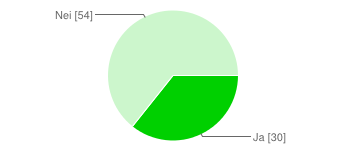
\includegraphics[scale=0.5]{charts/benytter-du-deg-av-noen-reiseplanlegger.png}
    \caption{Do you currently use any trip planners?}
\end{figure}

\begin{figure}[!h]
    \centering
    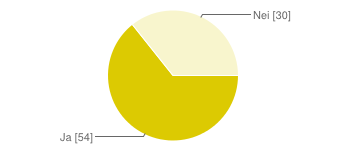
\includegraphics[scale=0.5]{charts/stoler-du-paa-reiseplanleggere.png}
    \caption{Do you trust trip planners?}
\end{figure}

\begin{figure}[!h]
    \centering
    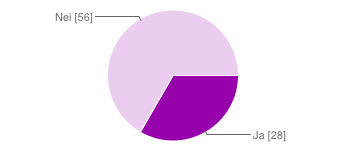
\includegraphics[scale=0.5]{charts/ville-du-betalt.png}
    \caption{Would you pay to use a good trip planner?}
\end{figure}

Though we have a small and biased sample, we'll make some observations based
on the data available. It seems that the assumption that people do not want to
pay for a trip planner was largely correct, potentially making advertisement a
good source of income. Furthermore, the majority of people trust trip planners
to function adequately, but do not currently use any; this may indicate that
what's lacking is a pleasant and unified user interface, although that is an
admittedly large assumption.

Taking a larger survey prior to making any big decisions would be a good idea;
in particular, it would seem pertinent to examine the large and financially
significant body of travelling professionals. However, at the very least,
what data we do have doesn't speak against the idea of a free-of-charge trip
planner being a potentially sound product.

\subsection{Initial Capital and Investment}

Given the strategies and observations laid out thus far, what we have is a
stand-alone software product with an uncertain potential for profit, and which
would have to be more or less complete (in terms of software development)
before it might enter the market. Therefore, it seems there are primarily two
realistic strategies for its initial development.

One possible strategy is to spend very little or nothing on initial
development of the product; this requires the developers to have another
source of income, and to take the risk of having no returns on their invested
effort. This may be a realistic strategy for students, or for a tightly knit
group of developers who believe in the product and are willing to spend their
free time on it.

Another strategy is to persuade a venture capitalist or an angel investor
that the product will make money in the future, and to have them finance the
development of the product. The disadvantage of this strategy is that the
investor will likely want significant returns in the event that the product
succeeds, given the high risk. Also, importantly, you would need to know or
get to know an investor.
